\section{Current System}

%Disposition
%kort introduction til hvad det er
%scenarier hvor bycyklen kan bruges
%hvem vedligeholder det
%cyklernes placering
%Positive erfaringer med bycyklen, ref god kilde

\bycykel is a bicycle system where people in Aalborg are able to borrow bicycles to travel around the city.
The system was started in September 2008 as part of the CIVITAS ARCHIMEDES project, which focuses on making bicycles more widely used \citep{misc:aalborgcykling}.
The bicycles can be found in stations located around the city of Aalborg, for exact placement of the bicycles see \figref{fig:CykelLokationer}.

\begin{figure}[h]
	\centering
	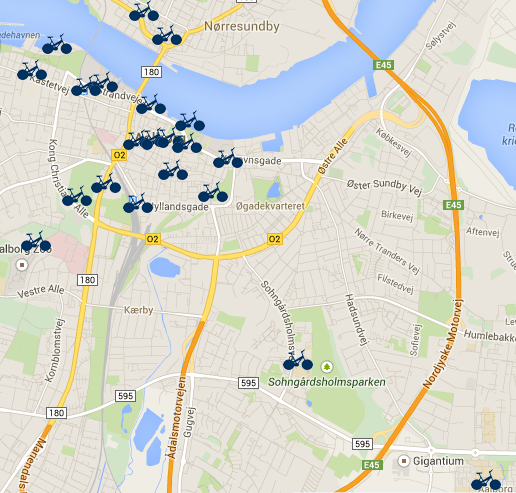
\includegraphics{analysis/CykelLokationer}
	\caption{Bicycle locations \citep{misc:aalborgbycykel}.}
	\label{fig:CykelLokationer}
\end{figure}

As can be seen, the bicycles are mostly located in the center of Aalborg, whereas fewer are placed in other areas.

In 2009, 135 bicycles was placed in Aalborg, and in 2012 this number had been increased to 200 bicycles \citep{misc:aalborgcykling}.

In order to borrow a bicycle, you need to go to one of the bicycle stations, deposit 20 DKK to unlock the bicycle, then return it to a station when you are done with the bicycle \citep{misc:aalborgbycykelregler}, where you will then retrieve your 20 DKK, which makes the system free to use.
The system is built on trust, because if people do not return the bicycles to a station when finished using them, the bicycles will gradually disappear.

\bycykel has had, as of 2012, success with their system. 
According to a report, if there had not been bicycles more than half of the users would have walked and 5 percent would have driven in a car instead \citep{misc:aalborgcykling}.
Furthermore, it shows that over three seasons the percentage of bicycles lost have been at maximum 11\% \citep{misc:aalborgcykling}.

As the bicycles are borrowed by depositing 20 DKK, it means that there is no additional monitoring of where the bicycles are located around the city, other than travelling around the city to locate the bicycles.
This poses the problem that it can be difficult for Aalborg Kommune and the potential users to know which stations have bicycles.
Another problem is if the bicycles are not returned to their stations after use, Aalborg Kommune has difficulty locating these misplaced bicycles.

On their website, it shows that a way for them of locating misplaced bicycles is through people reporting lost bicycles by way of SMS and voice mail, or by returning the bicycle themselves claiming the 20 DKK \citep{misc:aalborgbycykelmangler}.
However, if a lost bicycle is not reported or returned by someone, the bicycle is practically lost.
The company AFA JCDecaux is in charge of bicycle maintenance and storage during winter time and is also the company in charge of locating the lost bicycles \citep{misc:aalborgcykling}.

\subsection{Meeting with Aalborg Kommune}
In order to gain more information about \bycykelwithoutspace, a meeting with Aalborg Kommune was conducted. 
Through this meeting, various information was found, which is kept in mind when developing the system.

For the overview of bicycles, it was found that Aalborg Kommune has no control over the bicycles when they are placed at docks in Aalborg during the season.
The only information they get is if they see somebody bicycling in the city, or if a person makes a phone-call regarding a bicycle.

We also asked them if they had received any complaints, if so what those complaints consist of.
They said that the complaints they get is mostly about bicycles not being available, and also that they often see empty stations themselves.
This lead them to talk about how they are interested in gaining information the usage of the bicycles.
They thought that GPS tracking could be interesting, to monitor the bicycles and see how the bicycles are used, indicating that some admin statistical page is useful.

Additionally, we asked them if they have had any thoughts on booking of bicycles.
They told us that they had not thought of that but are open to the idea.
However, they can also see some cons for such a system, namely that it could become too restrictive for the user since bicycles have to be made unavailable for free use because of bookings.
They see that the usage of the bicycles as much more spontaneous instead of something the user plans to do.
However, when this was learned, the development of the booking part was well underway, and as such is kept as part of the system.
But the system is also not strictly developed for Aalborg Kommune alone, and as such, the booking system can still be of use.
Whereas, the admin part with statistics is aimed to be used by Aalborg Kommune.

%These problems could possibly be resolved, and to find inspiration to a solution, other existing systems are analysed.